\documentclass[a4paper,10pt]{article}

\usepackage[margin=0.7in]{geometry}
\usepackage[utf8]{inputenc}
\usepackage[english,german]{babel}

\usepackage{fancyhdr}
\usepackage{multicol}
\usepackage[parfill]{parskip}
\usepackage{graphicx}
\pagestyle{fancy}
\fancyhf{}
\rhead{Patrick Günthard}
\lhead{Spick Physikprüfung}
\rfoot{\thepage}
\lfoot{5. November 2016}
\begin{document}

\begin{multicols}{3}

  \section{Masseinheiten}
  \textit{jeweils nach SI}\\
  \begin{tabular}{|l|l|l|}
    \hline
    \textbf{Name} & \textbf{Bez.} & \textbf{SI} \\\hline
    Leistung & \(P\) & \(W\)\\\hline
  \end{tabular}

  \textit{Andere Einheiten}\\
  \(1 PS = 735,49875 W\)\\


  \section{Leistung}
  \textbf{Grundformel}\\
  \(P = \frac{\Delta E}{\Delta t} = \frac{\Delta W}{\Delta t} \)\\
  und\\
  \(P = \vec{F} * \vec{v}\)

  \section{Wirkungsgrad}
  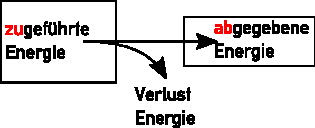
\includegraphics[width=5cm]{wirkungsgrad}\\
  \textbf{Grundformel}\\
  \(\eta = \frac{{\Delta {E_{ab}}}}{{\Delta {E_{zu}}}} = \frac{{{P_{ab}} \cdot \Delta t}}{{{P_{zu}} \cdot \Delta t}} \Rightarrow \eta = \frac{{{P_{ab}}}}{{{P_{zu}}}}\)
  \\
  Regel: \(\eta \leq 1\)
  \section{Energieerhaltungssatz}

  \section{Hydrostatik}
  \textbf{Grundfläche}\\
  \(\rho = \rho_{Fluessigkeit} * g * h\)\\
\end{multicols}

\end{document}
